\subsection{Méthode du maximum de vraisemblance}
\paragraph{Démonstration}
SAM


%b)
\paragraph{Echantillon, points candidats et fonction de vraisemblance}
La fonction nouvelle fonction \texttt{wblmle} nous permet de trouver un estimateur par la méthode du maximum de vraisemblance pour un échantillon aléatoire simple qui suit une loi de densité
$ f(x)= \frac{k}{c} \left(\frac{x}{c}\right)^{k-1} \exp \left[ -\left(\frac{x}{c}\right)^{k}\right] \mathbb{I}\{x \geq 0\}$ avec $k>0$ et $c>0$.
%b)
La première étape consiste à générer un échantillon $X_1,...,X_n$. Nous utilisons pour ce faire la fonction \texttt{wblrnd} avec un paramètre  $\theta$ au choix. Pour la suite de l'explication, posons $\theta = (k,c) = (3.7, 4.2)$. Nous construisons ensuite une grille de points candidats autour des valeurs de $k$ et $c$. La grille contient $101$ paires de point variant entre $(k-5, c-5)$ et $(k+5, c+5)$. Comme $k>0, c>0$, la borne inférieure est ramenée à $(0,0)$ pour les cas où $k<5$ ou $c<5$ (comme dans notre exemple). Pour chaque paire de points, nous calculons le logarithme de la fonction de vraisemblance depuis la fonction \texttt{wblloglike}~:
$$LL(\theta=(k,c)) = \sum_{i=1}^{n}{\ln(f(x_i;\theta=(k,c)))} = n\ln(k) - kn\ln(c) + \sum_{i=1}^{n}{\left[(k-1)\ln(x_i) - \left(\frac{x_i}{c}\right)^{k}\right]}$$

\paragraph{Estimateurs et maximum de vraisemblance} Une fois les 101 points candidats évalués, nous cherchons le maximum parmi eux pour déterminer le $k$ et $c$ qui lui correspondent et qui deviennent $\hat{k}_{MLE}$ et $\hat{c}_{MLE}$, nos estimateurs de choix. C'est ce qui correspond à l'étape analytique $\frac{\partial LL(\theta)}{\partial \theta} = 0$.

%c)
\paragraph{Un exemple} En exécutant \texttt{wblmle(1000, 4.2, 3.7)} (où $n = 1000$ le nombre de $X_i$, $c = 4.2$, $k = 3.7$), nous obtenons, par exemple, $\hat{k}_{MLE} = 3.6540$ et $\hat{c}_{MLE} = 4.1400$.
L'erreur quadratique totale pour ces valeurs est $ERT_{MLE} = (\hat{k}_{MLE} - k)^2 + (\hat{c}_{MLE} - c)^2 = 0.0057$.

%d)
\paragraph{500 \'Echantillons} La routine \texttt{MLE\_replicate} nous permet ensuite d'effectuez un certain nombre de réplications d'échantillons aléatoires simples et de calculer leurs $\hat{k}_{MLE}$, $\hat{c}_{MLE}$ et $ERT_{MLE}$ respectifs. Pour chacune des trois séries, nous calculons la moyenne et la variance. Les valeurs obtenues sont reprises dans la table~\ref{table:mle}.

\begin{table}[!ht]
\centering
\begin{tabular}{|l|l|l|}
\hline
				& Moyenne 	& Variance\\
\hline
$\hat{k}_{MLE}$ & 3.7069 	& 0.0096\\
$\hat{c}_{MLE}$ & 4.1998 	& 0.0023\\
$ERT_{MLE}$			& 0.0119	& 0.0002\\
\hline
\end{tabular}
\caption{Table des valeurs obtenues avec la méthode du maximum de vraisemblance pour 500 échantillons.}
\label{table:mle}
\end{table}

%e)
Pour chaque série, nous avons produit un box-plot et un histogramme. Les graphes relatifs à $\hat{k}_{MLE}$ se retrouvent à la figure~\ref{fig:kmle}, ceux de $\hat{c}_{MLE}$ à la figure~\ref{fig:cmle} et ceux de $ERT_{MLE}$ à la figure~\ref{fig:ertmle}.

\begin{figure}[!ht]
        \centering
        \begin{subfigure}[b]{0.5\textwidth}
                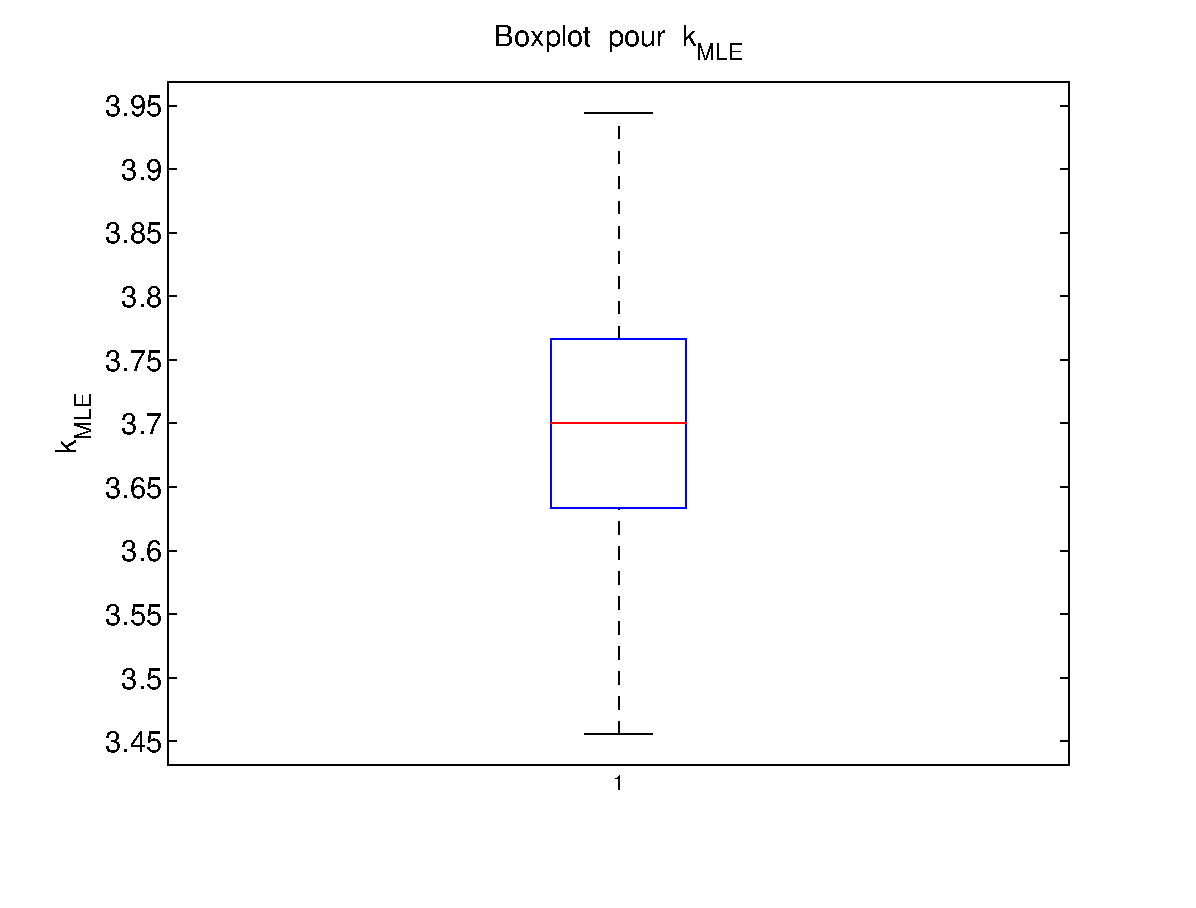
\includegraphics[width=\textwidth]{graphes/boxplot_kmle.eps}
        \end{subfigure}%
        ~
        \begin{subfigure}[b]{0.5\textwidth}
                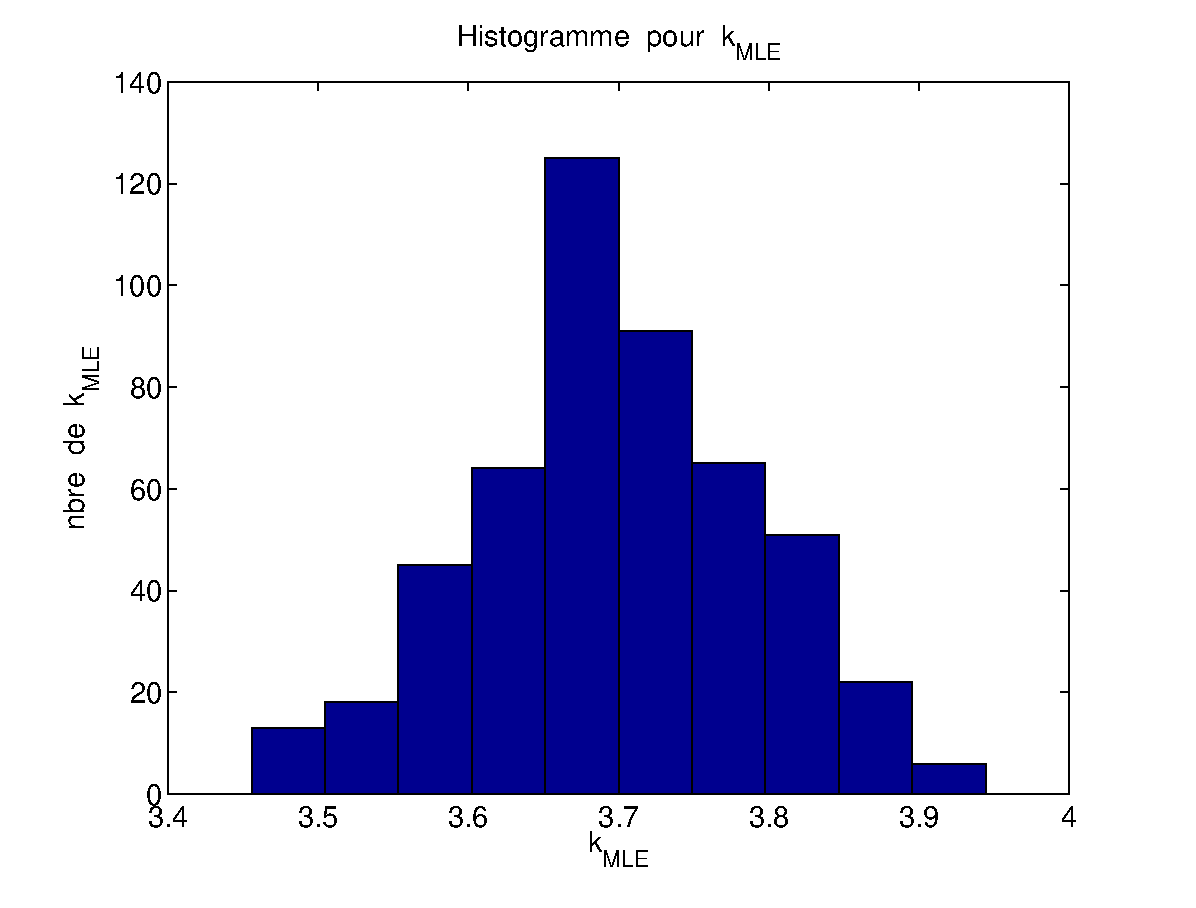
\includegraphics[width=\textwidth]{graphes/hist_kmle.eps}
        \end{subfigure}
        \caption{Graphes pour $\hat{k}_{MLE}$}\label{fig:kmle}
\end{figure}

\begin{figure}[!ht]
        \centering
        \begin{subfigure}[b]{0.5\textwidth}
                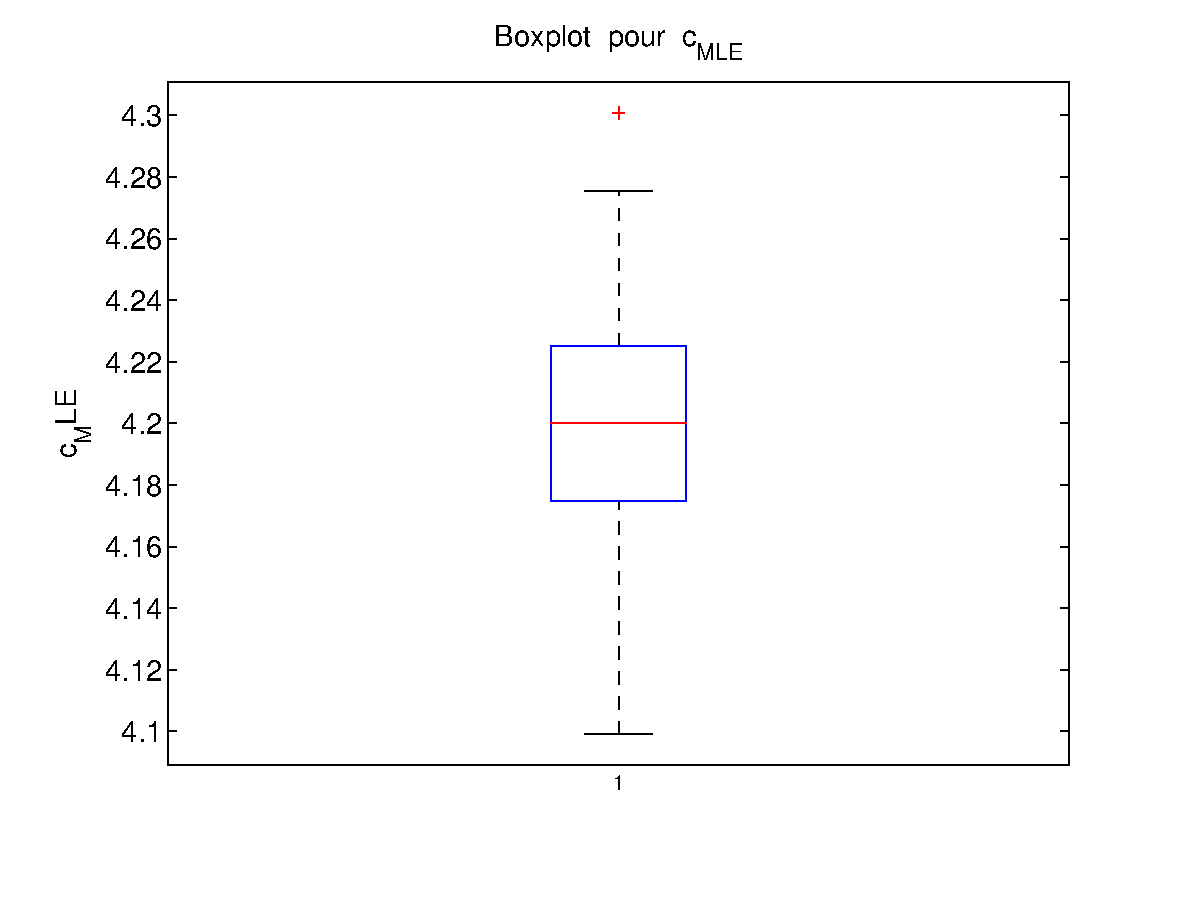
\includegraphics[width=\textwidth]{graphes/boxplot_cmle.eps}
        \end{subfigure}%
        ~
        \begin{subfigure}[b]{0.5\textwidth}
                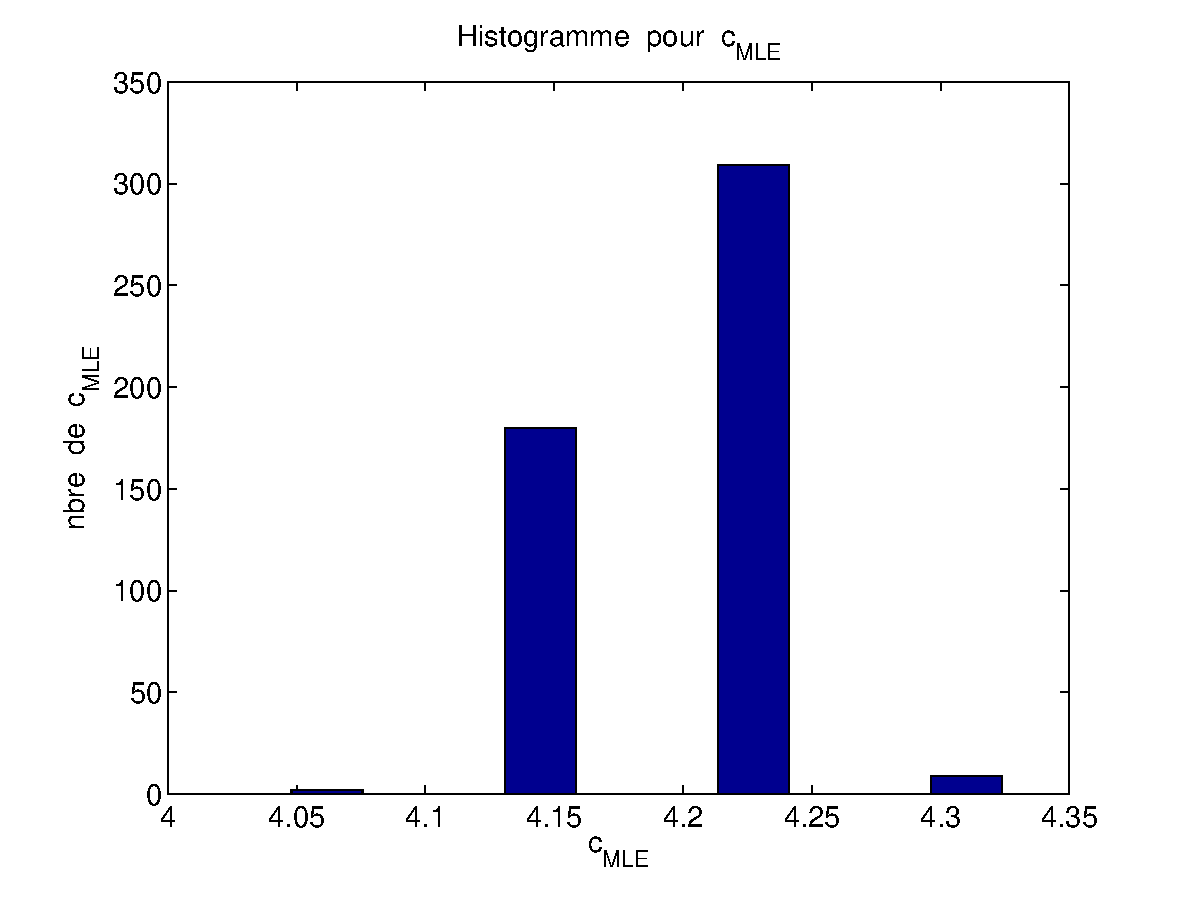
\includegraphics[width=\textwidth]{graphes/hist_cmle.eps}
        \end{subfigure}
        \caption{Graphes pour $\hat{c}_{MLE}$}\label{fig:cmle}
\end{figure}

\begin{figure}[!ht]
        \centering
        \begin{subfigure}[b]{0.5\textwidth}
                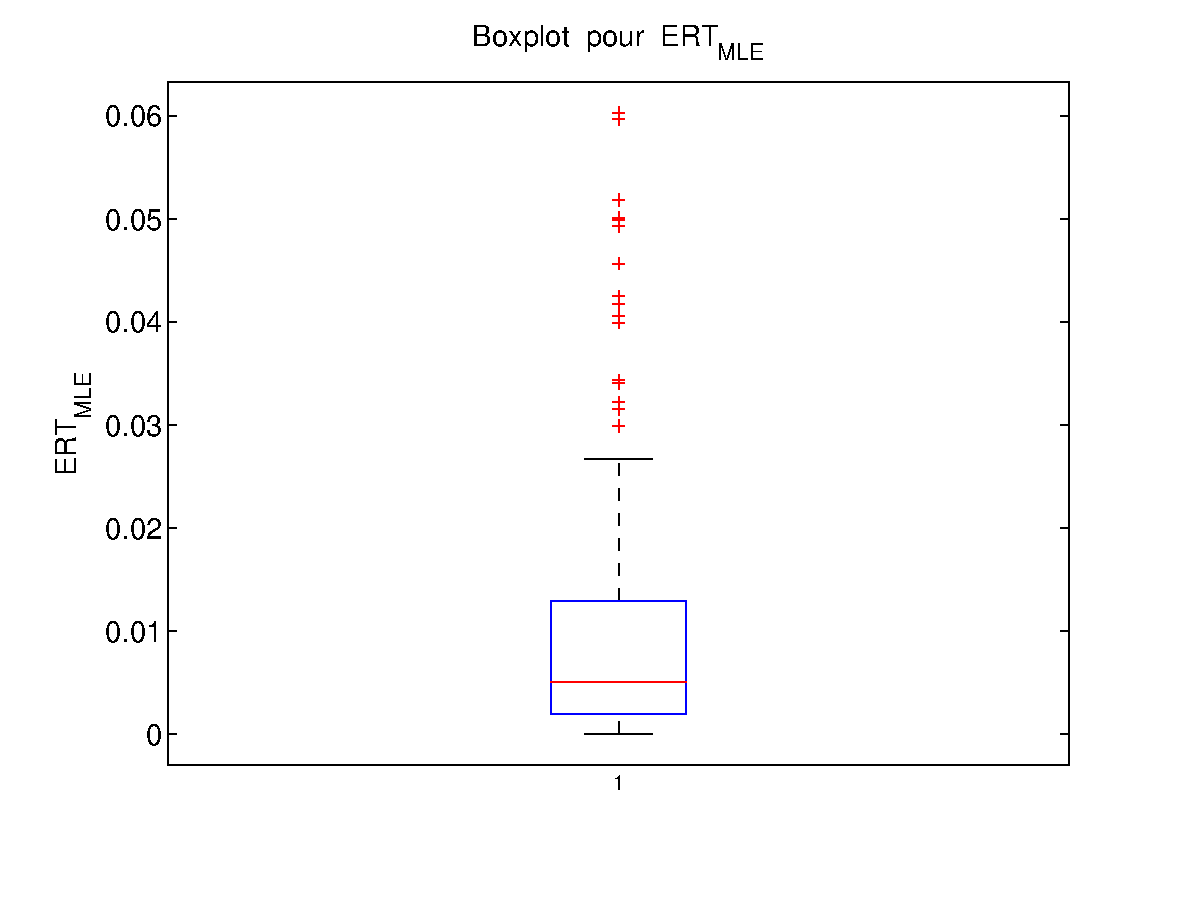
\includegraphics[width=\textwidth]{graphes/boxplot_ertmle.eps}
        \end{subfigure}%
        ~ 
        \begin{subfigure}[b]{0.5\textwidth}
                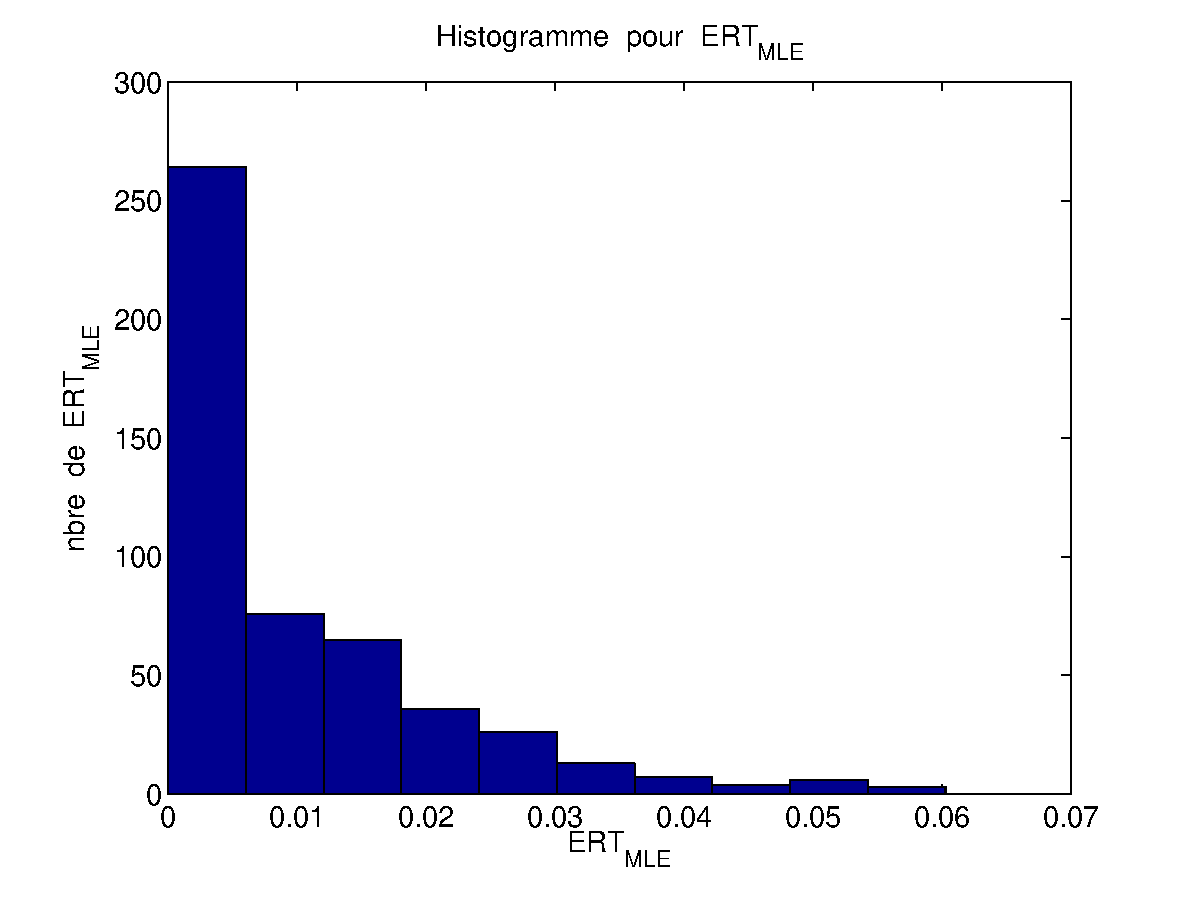
\includegraphics[width=\textwidth]{graphes/hist_ertmle.eps}
        \end{subfigure}
        \caption{Graphes pour $ERT_{MLE}$}\label{fig:ertmle}
\end{figure}

\paragraph{Biais, variance, consistence et distribution asymptotique}
\begin{align*}
biais(\hat{\theta}) &= \mathbb{E}(\hat{\theta}) - \theta \\
					&= \mathbb{E}(\bar{\theta}) - \theta
%					&= -0.0002
\end{align*}

\begin{align*}
\mathbb{V}(\hat{\theta}) 	&= \mathbb{V}(\bar{\theta})
\end{align*}

Consistence?
Distribution asymptotique?

% TODO
%f) Que pouvez-vous dire a propos du biais, de la variance, de la consistance et de la distribution asymptotique de votre estimateur ? Bien justifier votre réponse.

